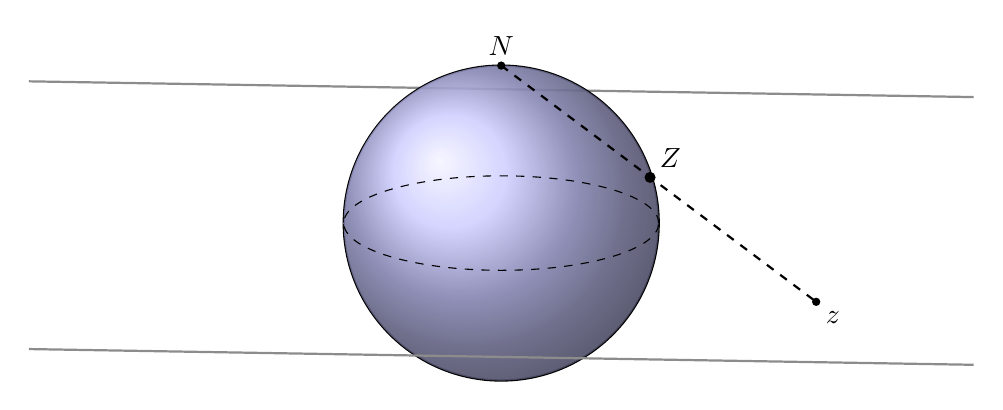
\begin{tikzpicture}

% upper plane
\draw[thick,gray!90]
  (-6,1.8) -- (6,1.6);
% \fill[gray!10,opacity=0.5]
%   (-6,1.8) -- (6,1.6) -- (6,-1.8) -- (-6,-1.6) -- cycle;

% Sphere
\draw[thick] (0,0) circle (2);
\shade[ball color=blue!25, opacity=0.9] (0,0) circle (2);
\fill (0,2) circle (1.5pt) node[above] {$N$};

% equator
\draw[dashed] (0,0) ellipse (2 and 0.6);

% lower plane
\draw[thick,gray!90]
  (-6,-1.6) -- (6,-1.8);

% projection
\fill (4,-1) circle (1.5pt) node[below right] {$z$};
\draw[dashed,thick] (0,2) -- (4,-1);

% sphere intersection
\fill (1.89,0.58) circle (2pt) node[above right] {$Z$};

\end{tikzpicture}
